% Review 1 deck -- compile with pdflatex (run twice). Self-contained: no other files needed.
\documentclass[aspectratio=169,11pt]{beamer}
% ---------------- theme (identical in review1.tex and review2.tex) ----------------
\usepackage[T1]{fontenc}
\usepackage{lmodern}
\usepackage{amsmath}
\usepackage{booktabs}
\usepackage{tabularx}
\usepackage{array}
\usepackage{listings}
\usepackage{tikz}
\usetikzlibrary{arrows.meta,positioning,calc,fit,backgrounds,shapes.geometric}

% ---------------------------------------------------------------- colours
\definecolor{paper}{HTML}{F3EDE2}
\definecolor{card}{HTML}{FBF8F2}
\definecolor{ink}{HTML}{1F1B16}
\definecolor{muted}{HTML}{6B6358}
\definecolor{rulec}{HTML}{CFC5B4}
\definecolor{accent}{HTML}{C8421B}
\definecolor{eventc}{HTML}{B7791F}
\definecolor{resc}{HTML}{1D5E5B}
\definecolor{volc}{HTML}{274B8F}
\definecolor{budc}{HTML}{5F6D1C}

\setbeamercolor{background canvas}{bg=paper}
\setbeamercolor{normal text}{fg=ink}
\setbeamercolor{structure}{fg=accent}
\setbeamercolor{alerted text}{fg=accent}
\setbeamercolor{itemize item}{fg=accent}
\setbeamercolor{itemize subitem}{fg=muted}
\setbeamertemplate{itemize item}{\small\raise1.2pt\hbox{\textbullet}}
\setbeamertemplate{itemize subitem}{\scriptsize\raise1pt\hbox{--}}
\setbeamertemplate{navigation symbols}{}

\setbeamertemplate{frametitle}{%
  \vspace{3pt}%
  {\color{accent}\scriptsize\ttfamily\bfseries \insertsubsection}\par
  {\color{ink}\Large\bfseries \insertframetitle}\par
  \vspace{2pt}{\color{ink}\rule{\textwidth}{0.6pt}}%
}
\setbeamertemplate{footline}{%
  \hspace{1.2em}{\color{muted}\tiny\ttfamily \footlinetext}\hfill
  {\color{accent}\tiny\ttfamily\bfseries \insertframenumber\,/\,\inserttotalframenumber}\hspace{1.2em}\vspace{8pt}%
}

% ---------------------------------------------------------------- helpers
\newcommand{\rs}{Rs.\,}
% \card{colour}{LABEL}{body}
\newcommand{\card}[3]{%
  \begin{tikzpicture}
    \node[draw=rulec, fill=card, line width=0.5pt, text width=\linewidth-14pt, inner sep=6pt, align=left] (c) {%
      {\color{#1}\scriptsize\ttfamily\bfseries #2}\par\vspace{2pt}\footnotesize #3};
    \draw[#1, line width=3pt] (c.north west) -- (c.north east);
  \end{tikzpicture}}

\tikzset{
  agent/.style={draw=#1, fill=card, line width=0.8pt, rounded corners=2pt, minimum height=9mm,
                text width=24mm, align=center, font=\scriptsize\bfseries},
  topbar/.style={draw=#1, line width=3pt},
  msg/.style={-{Stealth[length=2mm]}, line width=0.7pt, color=#1},
  lbl/.style={font=\tiny\ttfamily, fill=paper, inner sep=1pt},
}

\lstset{basicstyle=\ttfamily\tiny, keywordstyle=\color{accent}\bfseries, commentstyle=\color{muted}\itshape,
        stringstyle=\color{resc}, backgroundcolor=\color{card}, frame=single, rulecolor=\color{rulec},
        framesep=4pt, xleftmargin=4pt, xrightmargin=4pt, columns=fullflexible, keepspaces=true,
        showstringspaces=false, language=Python}

% ---------------------------------------------------------------- title page
\setbeamertemplate{title page}{%
  \begin{tikzpicture}[remember picture, overlay]
    \fill[ink] (current page.north west) rectangle ([yshift=-7mm]current page.north east);
    \node[anchor=west, text=paper, font=\tiny\ttfamily\bfseries] at ([xshift=8mm,yshift=-3.5mm]current page.north west)
      {CAMPUS FEST '26 \quad RESOURCE DESK \quad \reviewlabel};
  \end{tikzpicture}
  \vspace{10mm}
  {\color{accent}\footnotesize\ttfamily\bfseries \insertsubtitle}\par\vspace{4pt}
  {\color{ink}\fontsize{26}{28}\selectfont\bfseries \inserttitle}\par\vspace{10pt}
  {\color{ink}\rule{0.55\textwidth}{0.8pt}}\par\vspace{8pt}
  {\small \insertauthor}\par\vspace{6pt}
  {\footnotesize\color{muted} \insertinstitute}\par\vspace{4pt}
  {\footnotesize\color{muted}\ttfamily \insertdate}
}

\newcommand{\reviewlabel}{REVIEW 1}
\newcommand{\footlinetext}{Campus Fest Resource Allocation \textbullet{} Review 1}

\title{Campus Fest Resource Allocation System}
\subtitle{A MULTI-AGENT APPROACH \textbullet{} REVIEW 1}
\author{Member 1 (Reg.\ No.) \quad Member 2 (Reg.\ No.) \quad Member 3 (Reg.\ No.) \quad Member 4 (Reg.\ No.)}
\institute{Foundations of AI \textbullet{} Guide: Prof.\ \rule{25mm}{0.4pt} \textbullet{} Department of CSE, Your College}
\date{\today}

\begin{document}

% ------------------------------------------------------------------ 1
\begin{frame}[plain]
  \titlepage
\end{frame}

% ------------------------------------------------------------------ 2
\subsection{01 \textbullet{} THE CASE STUDY}
\begin{frame}{Problem \& motivation}
  \begin{columns}[T]
    \begin{column}{0.48\textwidth}
      \card{accent}{LIMITED RESOURCES}{%
        \begin{itemize}\setlength\itemsep{0pt}
          \item Classrooms, halls, labs, stages, ground
          \item Projectors, mics, speakers, food stalls, vehicles
          \item Volunteers (technical, security, registration, hospitality)
          \item One budget, one day (09:00--21:00)
        \end{itemize}}
    \end{column}
    \begin{column}{0.48\textwidth}
      \card{resc}{WHY IT IS HARD}{%
        \begin{itemize}\setlength\itemsep{0pt}
          \item Many events want the same venue \emph{at the same time}
          \item Priorities, capacities, budget, dependencies
          \item Requests keep arriving during the day
          \item Allocation must stay \emph{fair}
        \end{itemize}}
    \end{column}
  \end{columns}
  \vspace{4pt}
  \card{ink}{PROBLEM STATEMENT}{Autonomous agents negotiate venues, equipment, volunteers, budget and time
    for every event: no double booking, high priority first, a fair alternative or clear reason for the rest.}
\end{frame}

% ------------------------------------------------------------------ 3
\subsection{02 \textbullet{} PEAS FORMULATION}
\begin{frame}{PEAS}
  \begin{columns}[T]
    \begin{column}{0.49\textwidth}
      \card{accent}{P \textbullet{} PERFORMANCE MEASURE}{%
        Max.\ utilisation $U$, scheduled $S$, priority $P$, fairness $F$;
        min.\ conflicts $C$, budget overrun $B$.\\[3pt]
        $\text{Score}=w_1U+w_2S+w_3P+w_4F-w_5C-w_6B$\\[2pt]
        {\scriptsize\color{muted}$w=(0.15,\,0.30,\,0.30,\,0.25,\,1,\,1)$, $F$ = Jain's fairness index}}
      \vspace{4pt}
      \card{resc}{E \textbullet{} ENVIRONMENT}{%
        10 venues, 14 equipment items, 15 volunteers, \rs 80{,}000 budget, 12 hourly slots.
        Events: Hackathon, Cultural Night, Robotics, Sports, Music.}
    \end{column}
    \begin{column}{0.49\textwidth}
      \card{volc}{A \textbullet{} ACTUATORS}{%
        Allocate venue / equipment / volunteers, reserve a time slot, reject a request,
        reschedule, swap venue, preempt a lower-priority booking, propose and counter-propose.}
      \vspace{4pt}
      \card{budc}{S \textbullet{} SENSORS}{%
        Replies from other agents: resource availability and current holder, event requirements,
        time-slot availability, remaining budget, volunteer roster, priorities, existing conflicts.}
    \end{column}
  \end{columns}
\end{frame}

% ------------------------------------------------------------------ 4
\subsection{03 \textbullet{} ENVIRONMENT \& AGENT ANALYSIS}
\begin{frame}{Environment properties}
  \footnotesize
  \begin{tabularx}{\textwidth}{@{}l l X@{}}
    \toprule
    \textbf{Property} & \textbf{Campus fest} & \textbf{Justification} \\
    \midrule
    Observable    & Partially     & Each agent sees only its own ledger; others' state arrives via messages \\
    Deterministic & Mostly        & Same requests give the same allocation; arrivals are external \\
    Episodic      & Sequential    & Earlier bookings constrain later ones (and may be preempted) \\
    Static        & Dynamic       & New event requests arrive while the day is being planned \\
    Agents        & Multi-agent   & 5 agent types, cooperative with competing event agents \\
    Discrete      & Mostly        & Hourly slots, countable rooms, equipment and volunteers \\
    Known         & Mostly        & Resource catalogue and rules are known; event flexibility is private \\
    \bottomrule
  \end{tabularx}
  \vspace{8pt}

  \card{accent}{AGENT TYPE}{Utility-based agents: every Event agent scores options with its own
    deviation function, and the Coordinator minimises the priority-weighted total cost.}
\end{frame}

% ------------------------------------------------------------------ 5
\begin{frame}{Why multi-agent?}
  \begin{columns}[c]
    \begin{column}{0.52\textwidth}
      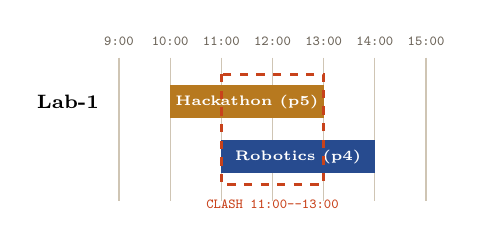
\begin{tikzpicture}[x=6.5mm, y=7mm]
        \foreach \h in {9,...,15} { \draw[rulec] (\h,0.2) -- (\h,-2.4); \node[font=\tiny\ttfamily, muted] at (\h,0.5) {\h:00}; }
        \node[anchor=east, font=\scriptsize\bfseries] at (8.8,-0.6) {Lab-1};
        \fill[eventc] (10,-0.3) rectangle (13,-0.9); \node[font=\tiny\bfseries, white] at (11.5,-0.6) {Hackathon (p5)};
        \fill[volc] (11,-1.3) rectangle (14,-1.9); \node[font=\tiny\bfseries, white] at (12.5,-1.6) {Robotics (p4)};
        \draw[accent, line width=1pt, dashed] (11,-0.1) rectangle (13,-2.1);
        \node[font=\tiny\ttfamily\bfseries, accent, anchor=north] at (12,-2.2) {CLASH 11:00--13:00};
      \end{tikzpicture}
      \vspace{8pt}

      {\footnotesize Event agent $\rightarrow$ Resource agent $\rightarrow$ \textcolor{accent}{\textbf{CONFLICT}}
       $\rightarrow$ Coordinator $\rightarrow$ negotiation $\rightarrow$ final allocation}
    \end{column}
    \begin{column}{0.44\textwidth}
      \card{muted}{CENTRALISED IF-ELSE}{One function sees everything and overwrites the loser.
        No ownership, no negotiation, and every new rule edits the same code.}
      \vspace{4pt}
      \card{accent}{MULTI-AGENT}{%
        \begin{itemize}\setlength\itemsep{0pt}
          \item Each desk owns its data and can refuse
          \item Events reveal private limits only when they reject an offer
          \item The Coordinator must negotiate: it holds no resources
          \item New agents or resources plug in without a rewrite
        \end{itemize}}
    \end{column}
  \end{columns}
\end{frame}

% ------------------------------------------------------------------ 6
\subsection{04 \textbullet{} ARCHITECTURE}
\begin{frame}{Multi-agent architecture}
  \centering
  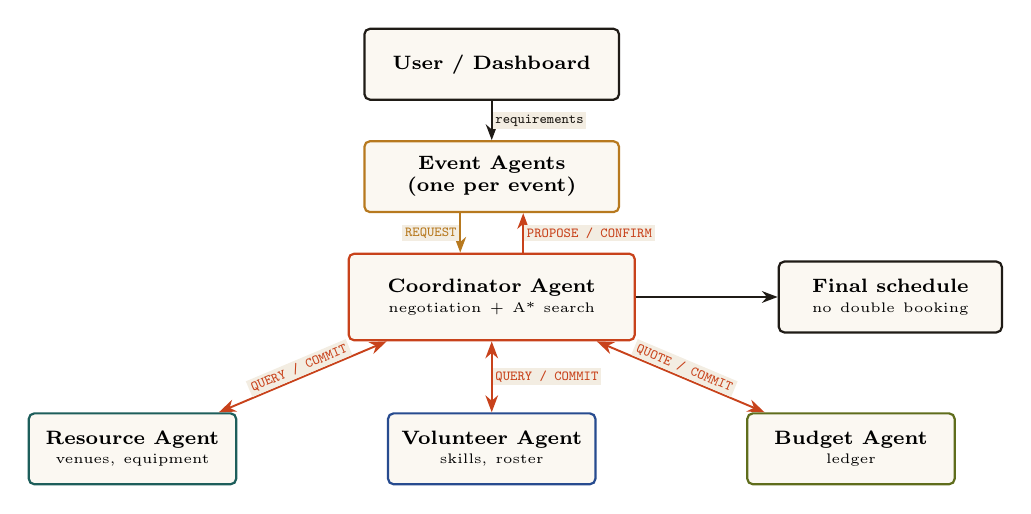
\begin{tikzpicture}[node distance=5mm and 7mm]
    \node[agent=ink, text width=30mm] (ui) {User / Dashboard};
    \node[agent=eventc, below=of ui, text width=30mm] (ev) {Event Agents (one per event)};
    \node[agent=accent, below=of ev, text width=34mm, minimum height=11mm] (co) {Coordinator Agent\\[-1pt]{\tiny\mdseries negotiation + A* search}};
    \node[agent=resc, below left=9mm and 14mm of co] (ra) {Resource Agent\\[-1pt]{\tiny\mdseries venues, equipment}};
    \node[agent=volc, below=9mm of co] (va) {Volunteer Agent\\[-1pt]{\tiny\mdseries skills, roster}};
    \node[agent=budc, below right=9mm and 14mm of co] (ba) {Budget Agent\\[-1pt]{\tiny\mdseries ledger}};
    \node[agent=ink, right=18mm of co, text width=26mm] (out) {Final schedule\\[-1pt]{\tiny\mdseries no double booking}};
    \draw[msg=ink] (ui) -- node[lbl, right] {requirements} (ev);
    \draw[msg=eventc] ([xshift=-4mm]ev.south) -- node[lbl, left] {REQUEST} ([xshift=-4mm]co.north);
    \draw[msg=accent] ([xshift=4mm]co.north) -- node[lbl, right] {PROPOSE / CONFIRM} ([xshift=4mm]ev.south);
    \draw[msg=accent, Stealth-Stealth] (co) -- node[lbl, sloped, above] {QUERY / COMMIT} (ra);
    \draw[msg=accent, Stealth-Stealth] (co) -- node[lbl, right] {QUERY / COMMIT} (va);
    \draw[msg=accent, Stealth-Stealth] (co) -- node[lbl, sloped, above] {QUOTE / COMMIT} (ba);
    \draw[msg=ink] (co) -- (out);
  \end{tikzpicture}
\end{frame}

% ------------------------------------------------------------------ 7
\begin{frame}{Agent responsibilities}
  \scriptsize
  \begin{tabularx}{\textwidth}{@{}>{\bfseries}l X X@{}}
    \toprule
    \textbf{Agent} & \textbf{Owns / perceives} & \textbf{Decides / says} \\
    \midrule
    {\color{eventc}Event}       & Its request, flexibility, private minimum volunteer ratio & Acceptable time windows; scores each option; ACCEPT / REJECT with a counter-constraint \\
    {\color{resc}Resource}      & Venue + equipment calendars & AVAILABLE / CONFLICT (+ holder) / ALTERNATIVE / ERROR; refuses double booking \\
    {\color{volc}Volunteer}     & Roster by skill and hour & OFFER / INSUFFICIENT; borrows from the general pool on shortage \\
    {\color{budc}Budget}        & Ledger of committed spending & APPROVE / REJECT each quote; refuses any over-budget commit \\
    {\color{accent}Coordinator} & Nothing, only the replies it receives & Detects clashes, preempts lower priority, runs A*, re-plans after counter-offers \\
    \bottomrule
  \end{tabularx}
  \vspace{8pt}

  \card{accent}{DESIGN RULE}{Agents interact \emph{only} through messages (FIPA-style performatives).
    The Coordinator cannot write into any other agent's state.}
\end{frame}

% ------------------------------------------------------------------ 8
\subsection{05 \textbullet{} ALGORITHMIC MODELLING}
\begin{frame}{Problem formulation: state, actions, goal}
  \begin{columns}[T]
    \begin{column}{0.47\textwidth}
      \card{accent}{STATE}{%
        $n = \langle i,\ (o_1,\dots,o_i)\rangle$\\
        events $1..i$ are decided; each $o_k$ is an option
        (venue, slot, equipment, volunteers, cost) or \textsc{Reject}.
        Plus: calendars, rosters, budget remaining.}
      \vspace{4pt}
      \card{volc}{ACTIONS}{%
        \textsc{Allocate} an option \textbullet{} \textsc{Reject} \textbullet{}
        \textsc{Swap} venue \textbullet{} \textsc{Reschedule} slot \textbullet{}
        \textsc{Negotiate} (propose / counter) \textbullet{} \textsc{Preempt}}
    \end{column}
    \begin{column}{0.5\textwidth}
      \card{resc}{GOAL TEST: ALL EVENTS DECIDED AND}{%
        $\begin{array}{@{}l@{\quad}l@{}}
          v_a = v_b \Rightarrow [s_a,e_a)\cap[s_b,e_b)=\emptyset & \text{venue}\\[2pt]
          \sum_{k \in \text{overlap}} q_{k,r} \le \text{free}_r & \text{pooled items}\\[2pt]
          \sum_k \text{cost}_k \le B_{\text{left}} & \text{budget}\\[2pt]
          e_d \le s_x \ \ \forall\, d \in \text{deps}(x) & \text{dependencies}\\[2pt]
          \text{cap}(v_k) \ge \text{participants}_k & \text{capacity}
        \end{array}$}
    \end{column}
  \end{columns}
  \vspace{4pt}
  {\footnotesize\color{muted} A constraint-satisfaction problem with an optimisation objective, solved by informed search.}
\end{frame}

% ------------------------------------------------------------------ 9
\begin{frame}{Search strategy: A*}
  \begin{columns}[c]
    \begin{column}{0.5\textwidth}
      \card{accent}{EVALUATION}{%
        $f(n) = g(n) + h(n)$\\[4pt]
        $g(n) = \sum_{\text{allocated}} p_k\, d_k \;+\; \sum_{\text{rejected}} 25\,p_k$\\[4pt]
        $h(n) = \sum_{\text{undecided}} \min\!\big(\min_o p_k d_o,\ 25\,p_k\big)$}
      \vspace{4pt}
      \card{resc}{WHY IT IS CORRECT}{%
        $h$ ignores clashes (a relaxation), so it never overestimates: it is admissible,
        and A* returns the minimum-cost allocation. Events are expanded by priority,
        with dependencies first.}
    \end{column}
    \begin{column}{0.47\textwidth}
      \centering
      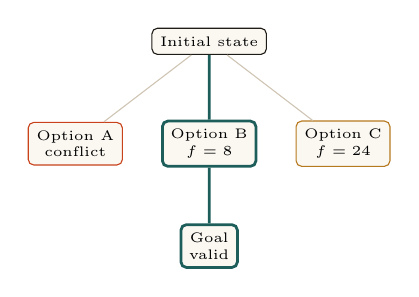
\begin{tikzpicture}[level distance=13mm, sibling distance=17mm,
          every node/.style={draw=rulec, fill=card, rounded corners=2pt, font=\tiny, align=center, inner sep=3pt}]
        \node[draw=ink] {Initial state}
          child { node[draw=accent] {Option A\\conflict} edge from parent[draw=rulec] }
          child { node[draw=resc, line width=1pt] {Option B\\$f=8$}
            child { node[draw=resc, line width=1pt] {Goal\\valid} edge from parent[draw=resc, line width=1pt] }
            edge from parent[draw=resc, line width=1pt] }
          child { node[draw=eventc] {Option C\\$f=24$} edge from parent[draw=rulec] };
      \end{tikzpicture}
      \vspace{4pt}

      {\scriptsize The pruned branch violates a constraint; the expensive branch is never expanded
      because B reaches the goal with a lower $f$.}
    \end{column}
  \end{columns}
\end{frame}

% ------------------------------------------------------------------ 10
\begin{frame}{Deviation and the priority rule}
  \begin{columns}[T]
    \begin{column}{0.47\textwidth}
      \card{eventc}{EVENT AGENT'S DEVIATION D}{%
        \begin{tabular}{@{}ll@{}}
          same type, other room & $+2$ \\
          fallback venue type   & $+4$ \\
          per hour shifted      & $+3$ \\
          missing volunteers    & $+10\times$ fraction \\
          cost (tie-breaker)    & $+\text{cost}/50000$ \\
        \end{tabular}}
      \vspace{4pt}
      \card{accent}{PRIORITY RULE}{Step cost $=p\times d$. Displacing a priority-5 event costs
        $2.5\times$ as much as displacing a priority-2 event, so the lower priority moves.}
    \end{column}
    \begin{column}{0.5\textwidth}
      \card{resc}{WORKED EXAMPLE: BOTH WANT LAB-1}{%
        \begin{tabular}{@{}lr@{}}
          Robotics $\rightarrow$ Lab-2 \quad ($4\times2$) & \textbf{8} \\
          Hackathon $\rightarrow$ Lab-2 \quad ($5\times2$) & 10 \\
          Robotics shifted +2\,h \quad ($4\times6$) & 24 \\
          Reject Robotics \quad ($25\times4$) & 100 \\
        \end{tabular}\\[4pt]
        A* picks the cheapest consistent plan: Hackathon keeps Lab-1 and Robotics moves to Lab-2.}
    \end{column}
  \end{columns}
\end{frame}

% ------------------------------------------------------------------ 11
\subsection{06 \textbullet{} CONFLICT RESOLUTION}
\begin{frame}{Conflict resolution example}
  \centering
  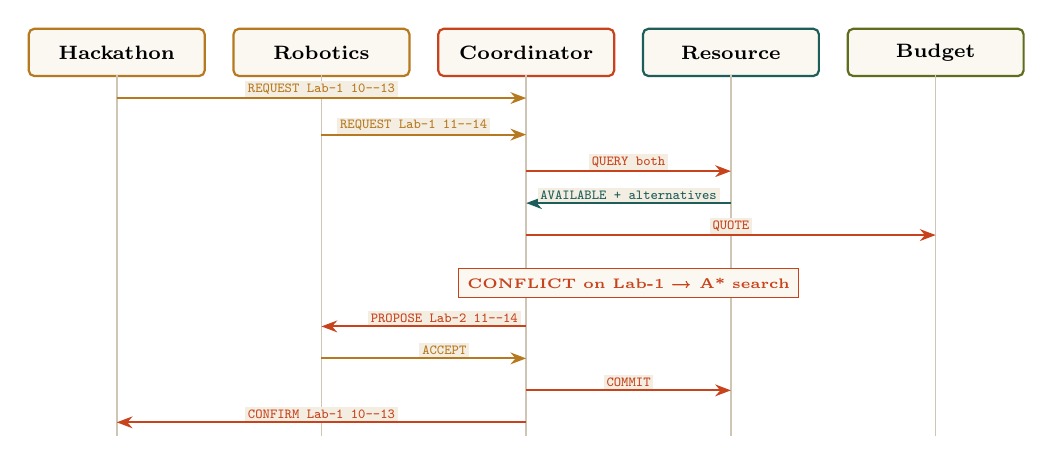
\begin{tikzpicture}[x=10mm, y=5.8mm]
    \foreach \x/\n/\col in {0/Hackathon/eventc, 2.6/Robotics/eventc, 5.2/Coordinator/accent, 7.8/Resource/resc, 10.4/Budget/budc} {
      \node[agent=\col, text width=20mm, minimum height=6mm] at (\x,0) {\n};
      \draw[rulec, line width=0.6pt] (\x,-0.5) -- (\x,-8.4);
    }
    \draw[msg=eventc] (0,-1) -- node[lbl, above] {REQUEST Lab-1 10--13} (5.2,-1);
    \draw[msg=eventc] (2.6,-1.8) -- node[lbl, above, pos=0.45] {REQUEST Lab-1 11--14} (5.2,-1.8);
    \draw[msg=accent] (5.2,-2.6) -- node[lbl, above] {QUERY both} (7.8,-2.6);
    \draw[msg=resc] (7.8,-3.3) -- node[lbl, above] {AVAILABLE + alternatives} (5.2,-3.3);
    \draw[msg=accent] (5.2,-4) -- node[lbl, above] {QUOTE} (10.4,-4);
    \node[draw=accent, fill=card, font=\tiny\bfseries, text=accent, align=center] at (6.5,-5.05) {CONFLICT on Lab-1 \textrightarrow\ A* search};
    \draw[msg=accent] (5.2,-6) -- node[lbl, above, pos=0.4] {PROPOSE Lab-2 11--14} (2.6,-6);
    \draw[msg=eventc] (2.6,-6.7) -- node[lbl, above, pos=0.6] {ACCEPT} (5.2,-6.7);
    \draw[msg=accent] (5.2,-7.4) -- node[lbl, above] {COMMIT} (7.8,-7.4);
    \draw[msg=accent] (5.2,-8.1) -- node[lbl, above] {CONFIRM Lab-1 10--13} (0,-8.1);
  \end{tikzpicture}
  \vspace{2pt}

  {\footnotesize \textbf{Result:} Hackathon $\rightarrow$ Lab-1 10:00--13:00 \quad
   Robotics $\rightarrow$ Lab-2 11:00--14:00 \quad (negotiated, not overwritten)}
\end{frame}

% ------------------------------------------------------------------ 12
\begin{frame}{Approaches we will compare}
  \footnotesize
  \begin{tabularx}{\textwidth}{@{}l X X X@{}}
    \toprule
     & \textbf{Greedy} & \textbf{A* search} & \textbf{Multi-agent negotiation} \\
    \midrule
    Idea        & Highest priority grabs its best free option & Optimal combination of all options & Agents query, propose, counter-propose and commit \\
    Look-ahead  & None                      & Full (admissible $h$)          & A* inside each negotiation round \\
    Optimal?    & No                        & Yes, for the given options     & Yes, plus private constraints \\
    Weakness    & Can starve later events   & Needs every option up front    & More messages \\
    Handles     & Priority only             & Priority, budget, dependencies & Plus counter-offers, preemption, dynamic arrivals \\
    \bottomrule
  \end{tabularx}
  \vspace{10pt}

  \card{accent}{HYPOTHESIS TO TEST IN REVIEW 2}{Negotiation with A* never scores below greedy, and beats it
    whenever an early choice blocks a later event (for example, by spending the budget).}
\end{frame}

% ------------------------------------------------------------------ 13
\subsection{07 \textbullet{} EXPECTED OUTPUT}
\begin{frame}{Expected output}
  \begin{columns}[T]
    \begin{column}{0.46\textwidth}
      \begin{itemize}\footnotesize
        \item Conflict-free timetable for every venue and hour
        \item Equipment IDs and volunteer IDs per event
        \item For each moved event: \emph{what} changed and \emph{why}
        \item For each rejected event: the exact reason
        \item Full log of the agent conversation
        \item Score and comparison: greedy vs A*
        \item Dashboard: live board, booking form, scenarios
      \end{itemize}
    \end{column}
    \begin{column}{0.52\textwidth}
      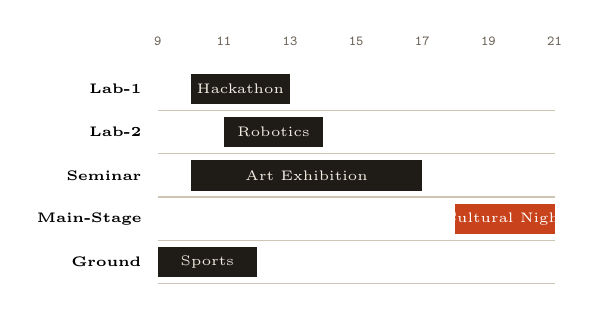
\begin{tikzpicture}[x=4.2mm, y=5.5mm]
        \foreach \h in {9,11,...,21} { \node[font=\tiny\ttfamily, muted] at (\h-9,0.6) {\h}; }
        \foreach \v/\y in {Lab-1/0, Lab-2/1, Seminar/2, Main-Stage/3, Ground/4} {
          \node[anchor=east, font=\tiny\bfseries] at (-0.2,-\y-0.5) {\v};
          \draw[rulec] (0,-\y-1) -- (12,-\y-1);
        }
        \fill[ink] (1,-0.15) rectangle (4,-0.85);  \node[font=\tiny, paper] at (2.5,-0.5) {Hackathon};
        \fill[ink] (2,-1.15) rectangle (5,-1.85);  \node[font=\tiny, paper] at (3.5,-1.5) {Robotics};
        \fill[ink] (1,-2.15) rectangle (8,-2.85);  \node[font=\tiny, paper] at (4.5,-2.5) {Art Exhibition};
        \fill[accent] (9,-3.15) rectangle (12,-3.85); \node[font=\tiny, white] at (10.5,-3.5) {Cultural Night};
        \fill[ink] (0,-4.15) rectangle (3,-4.85);  \node[font=\tiny, paper] at (1.5,-4.5) {Sports};
      \end{tikzpicture}
      \vspace{4pt}

      {\scriptsize\color{muted} Illustrative timetable (venue $\times$ hour).}
    \end{column}
  \end{columns}
\end{frame}

% ------------------------------------------------------------------ 14
\begin{frame}[plain]
  \vfill
  \centering
  {\color{accent}\ttfamily\small THANK YOU}\par\vspace{6pt}
  {\fontsize{30}{32}\selectfont\bfseries Questions?}\par\vspace{10pt}
  {\color{ink}\rule{0.3\textwidth}{0.8pt}}\par\vspace{8pt}
  {\footnotesize\color{muted} Five agents \textbullet{} one fest day \textbullet{} zero double bookings}
  \vfill
\end{frame}

\end{document}
